\chapter{Background}\label{ch:background}
%************************************************ 

\section{Neural networks as classifiers}

	One of the most popular use cases of \acs{ANN}s is supervised learning; what distinguishes it from unsupervised learning is the existence of labeled examples that guide the learning stage, against the need to infer all information. Supervised learning can be further divided into classification and regression: the former aims to split a set of data into two or more groups, while the latter is more of a function approximation. Since our job will consist in recognizing several types of \acs{EEG} patterns, the discussion will focus on the particular details of classification from here on.

	A neural network, in its most basic form, is made of simple processing units (called \textit{neurons}) distributed among three kinds of layers:

	\begin{itemize}

		\item
		Input layer: with as many neurons as characteristics describing a single sample. Each unit receives the value of its corresponding characteristic as is. Depending on the problem (and not just for this sort of model), it may be useful to preprocess the data so as not to bias the model.

		\item
		Output layer: the number of possible outputs dictates its number of neurons. Only one of them can be active at a time, indicating the answer of the neural network to the classification question.

		\item
		Hidden layers: these are inserted between the previous two. Their quantity ranges from one to hundreds in the most extreme applications, and their interactions yield the predictive ability of the model.

	\end{itemize}

	A typical vanilla feed-forward neural network contains directed connections between its different layers, but not between components of the same layer. Also, the term \textit{feed-forward} implies that there are no cycles in the graph of the network, and so the information moves from the input to the output through the hidden layers. The way in which this information flows is defined by the \textit{activation function} (the response of a neuron from an input number) as well as the \textit{weights} of the connections between neurons: although it is frequent to have fully-connected layers, it does not mean that one unit passes the same value to all the other units it points to, or even that they are not null; finding it out is precisely the task of the learning algorithm.

\newpage

	To get a better picture of the concept, the following figure illustrates a generic model with one hidden layer:

	\vspace{0.2cm}

	\begin{figure}[bth]

        \myfloatalign
        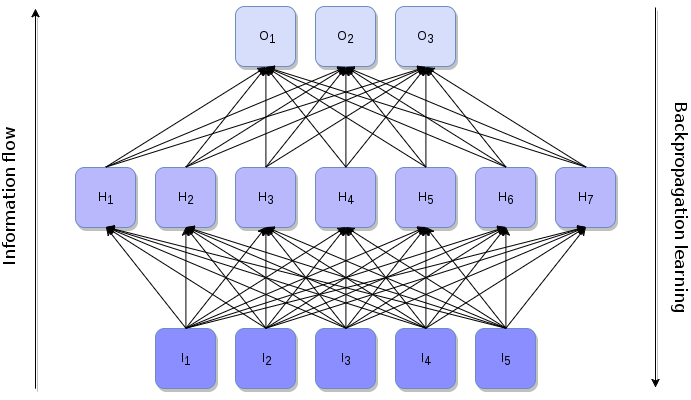
\includegraphics[width=0.9\textwidth]{gfx/NeuralNetwork.png}
        \caption{A neural network with one hidden layer.}

    \end{figure}

    We can see that the hidden layer has its neurons labeled $H_i$. The input layer is represented by the $I_i$ units and the output layer corresponds to the different $O_i$. 

    This image introduces another new concept: \textit{backpropagation}. Whereas the information is transformed by means of the weights and transmitted forward, the adjustment of those weights also needs of a propagation in the opposite direction. To sum it up, backpropagation has two main steps:

    \begin{enumerate}

    	\item
    	Propagation. Generate predictions for the training examples, then calculate the error at the output layer; a common error measure is the squared difference between the actual value and the expected value. Afterwards, recursively propagate the error calculations to the successive hidden layers taking into acount the already computed error values, until the input layer is reached.

    	\item
    	Weight update. Multiply the value of the activation function of each neuron and its error obtained in the first step. This is called the \textit{gradient} in \textit{Gradient Descent}. Finally, subtract a fraction of this gradient from the weight; that fraction (\textit{learning rate}) has a significant effect on the process, for a value too high can cause the algorithm to jump over a local minimum without reaching it, and a value too low can overextend the training time.

    \end{enumerate}

    The above procedure is repeated until the model's performance is adequate. If we wish to speed it up with a reasonable tradeoff in quality, we can use not the whole training set for each iteration but smaller subsets called \textit{batches} (\textit{Stochastic Gradient Descent}). This allows us to maintain enough generalization while at the same time reducing the cost of gradient computation \cite{lecun-dl}.

    A problem related to backpropagation is the \textit{vanishing gradient}, which only occurs in the training stage of neural networks. Because of the chain rule used to propagate the error through the layers, if the activation function has a near-zero derivative at some points, the gradient will approach that value too. In worst-case scenarios, it results in a practical standstill of the training.

    Multiple solutions have been proposed in the past few years, and research on the topic is still ongoing. A few popular activation functions as of now include:

    \begin{itemize}

    	\item
    	\textit{Hyperbolic tangent}: the classic, due to it being bounded, which increases the efficiency of the training. However, its shape at both ends produces the vanishingly small gradients.

    	\item
    	\textit{\ac{ReLU}}: defined by $f(x) = 0$ if $x \leq 0$ and $f(x) = x$ if $x > 0$. It avoids small gradients for high input values and makes networks sparser with its negative part (accounting again for more efficiency). The downside is the \textit{dying} \acs{ReLU}, in which some neurons become perpetually inactive.

    	\item
    	\textit{Leaky \acs{ReLU}}: one of the variants of \acs{ReLU} which tries to avoid inactive neurons by setting $f(x)$ for negative $x$ to $0.01x$ instead of $0$. Its generalization is the \textit{Parameterized ReLU} \cite{delv-deep-relu,deep-res-relu}.

    	\item
    	\textit{\ac{ELU}} \cite{elu}: another recent alternative that replaces the horizontal section of the \acs{ReLU} with an exponential function.

    \end{itemize}

    These functions can be observed in the following figure:

    \vspace{0.2cm}

    \begin{figure}[bth]

        \myfloatalign
        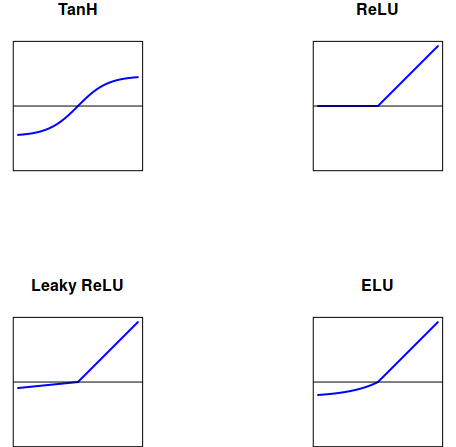
\includegraphics[width=0.7\textwidth]{gfx/ActivationFunctions.png}
        \caption{Four of the most popular activation functions.}

    \end{figure}

    In general, as the complexity of a model grows, so does the difficulty of its training. Neural networks are, in theory, capable of approximating every possible function, and this comes at a price: some of the following common issues in machine learning \cite{nn-atc} have increased consequences.

    \begin{itemize}

    	\item
    	Limited data: without delving too much into the underlying theory, the more powerful a model is, the more training samples are needed in a substantial proportion. Coupled with it, the smaller the training set, the smaller the chance it will represent the whole population.

    	\item
    	Imbalanced data: when there are far more examples of one or more classes than of the rest, we speak of imbalance. Apart from not representing the population, this phenomenon can even bias a classifier in a way that it only outputs one class, as it seems the best way to minimize the error.

    	\item
    	Incomplete data: this is the case when the available samples have missing values. In this situation there are two options: either we discard incomplete fields from across all samples or we try to infer them.

    	\item
    	High dimensionality: linking with the first bullet point, powerful models can suffer of \textit{overfitting} with limited and/or high-dimensional samples. The latter can cause the model to just learn the available data ``by heart'' and fail to generalize to new examples. Even leaving extreme cases aside, the number of features directly impacts the time required for training.

    \end{itemize}

    It is clear that we must minimize the hurdles posed by the data, and also make sure we pick the right parameters. For this second task, we have \acf{EA}.

\section{Evolutionary algorithms}

	Evolutionary algorithms are iterative procedures that take a population of feasible solutions to a problem and try to progressively find the best possible answer by mimicking nature in its selection process. 

	Because they are general-purpose metaheuristics, they find use in fields as disparate as computer science, medicine, economics or cryptography, among many others. In the business at hand, they will serve as neural network optimizers, in addition to feature selectors in a preliminar step.

\newpage

	The kind of \acs{EA}s we will be using are known as \textit{genetic algorithms}. Now, if we analyze them, we find they have several main pieces:

	\begin{itemize}

		\item
		Individual: a potential solution to a problem, represented in an adequate manner.

		\item
		Population: a set of individuals for a given iteration (\textit{generation}).

		\item
		Fitness: every genetic algorithm has one or more fitness functions which evaluate the quality of an individual. It can be the most expensive operation, depending on the situation.

		\item
		Selection process: the creation of new individuals (\textit{offspring}) needs a set of parents. The selection process chooses them based on some criteria, usually involving the fitness.

		\item
		Crossover operator: once we have a list of potential parents, this operator defines how to create \textit{offspring} that resemble them in some way.

		\item
		Mutation operator: in order to maintain diversity, random mutations are introduced with a certain probability.

		\item
		Replacement: how the old population and the offspring set will be used to create a new population.

	\end{itemize}

	Strong emphasis is placed on a solid balance between finding novel solutions and improving the best ones yet, also known as the \textit{exploration-exploitation tradeoff}. Hence, all the pieces as a whole must attain a delicate synergy. With that in mind, let us go into a bit more detail in the next sections.

	\subsection{Individuals}

		The individuals of a genetic algorithm may be represented in a variety of ways. It is crucial to find the best suited for our needs, as it will not only impact time and space efficiency but also the overall performance of the optimization, enabling some genetic operators and discarding others.

		For example, in feature selection we could code our solutions as a binary vector in which the ones represent active features and the zeros inactive features. Alternatively, we could just keep a list of the indices of active features; this would use less memory but also make some very simple operators in binary codification way more convoluted to implement.

		That said, common representations include binary, order-based and real-valued. The first already exemplified, order-based is natural in \textit{Travelling Salesman Problem}-like cases and real-valued can be found in numerical function optimization.

	\subsection{Population}

		Population size must have an equilibrium between enough individuals to explore the solution space and not too many of them, which would lead to excessive running times.

		Another relevant discussion is how to initialize the first set of individuals. For the sake of a good exploration, it should include a decent portion of the search space, often taking advantage of randomness.

	\subsection{Fitness}

		Fitness measures, both in type and in number, depend on what aspect of a problem we want to tackle. 

		If we hope to find a global maximum or minimum in a complex function, the fitness will just compute the value at a given point. If we want to choose from a set of features, the evaluation will need to assess how good a subset is by training and testing a machine-learning model; similarly, if we wanted to further optimize that model, we would need to try many variations of its parameters.

		However, suppose we can't decide on what we prefer to improve: for instance, we want a solution to be as accurate as possible, but we want it to be simple, too. This is when \textit{multiobjective optimization} comes in: instead of returning the best candidate, we accept a compromise between the two criteria and return a list of candidates that are not better or worse than the others. They just score well in both measures but in different proportions.

	\subsection{Selection}

		Parent selection process is one of the keys for the success or failure of the algorithm. Since it is a problem-independent part of the algorithm, in contrast with the more specific crossover and mutation operators, we can reduce our choices to a handful of classic techniques \cite{selection-ga}:

		\begin{itemize}

			\item
			Proportional: the probability of picking an individual is driven by its relative fitness with respect to the overall sum.

			\item
			Tournament: $n$ random individuals are set side by side and compared by fitness score, after which the best is taken. Repeat until the parent quota is met.

			\item
			Ranking (any kind): with the population sorted by fitness, it assigns order-based probabilities following some function. The catch here is that the probabilities are not directly related to the measured quality of the solutions, which allows for more control over convergence-exploration.

			\item
			Randomized: little to no influence of fitness in the decision.

		\end{itemize}

	\subsection{Crossover}

		A highly representation-dependent operator, there exist a plethora of options. As it is unfeasible to list them all, even just the most relevant ones, we will limit this section to the kinds we will use. The only prerequesite is that they offer a degree of continuity from parent to offspring.

		\subsubsection{In binary representation}

			Like we mentioned earlier, a binary representation consists of a series of zeros and ones. While not the most memory-efficient alternative, it results in fairly straightforward yet powerful operators:

			\begin{itemize}

				\item
				Single-point: choose a random position between the first and the last. To each of its sides we only add the elements of a single parent.

				\vspace{0.2cm}

			    \begin{figure}[bth]

			        \myfloatalign
			        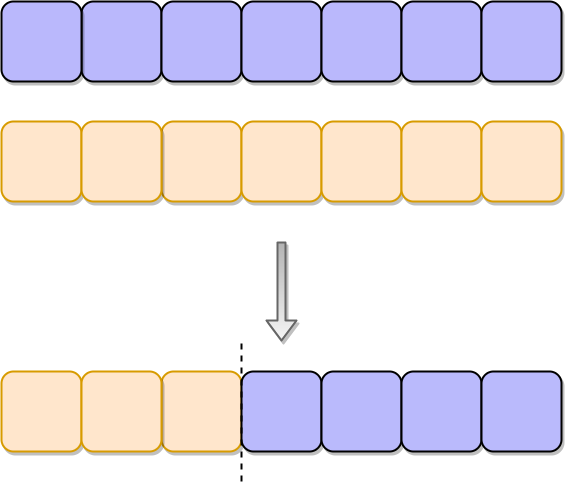
\includegraphics[width=0.5\textwidth]{gfx/SinglePointCrossover.png}
			        \caption{Single-point crossover example.}

			    \end{figure}

			    \item
			    Double-point: this time, generate two random positions. Use them to alternate the two parents' elements. Note that this idea can be extended to $n$-point crossovers.

			    \vspace{0.2cm}

			    \begin{figure}[bth]

			        \myfloatalign
			        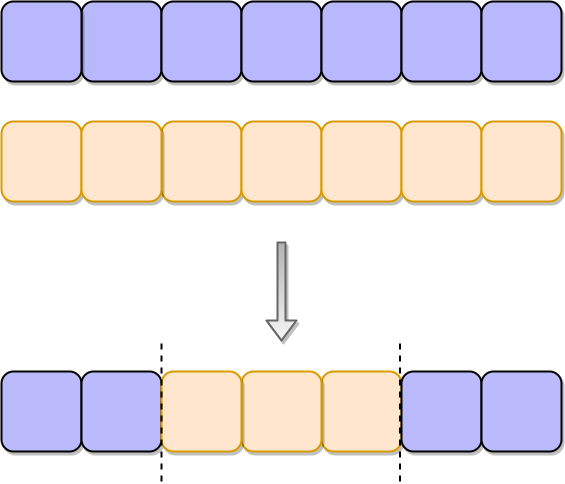
\includegraphics[width=0.5\textwidth]{gfx/DoublePointCrossover.png}
			        \caption{Double-point crossover example.}

			    \end{figure}

			    \item
			    Uniform (UX): choose a uniform real number between 0 and 1 and use it to decide which of the two parents the $ith$ bit will come from. From a practical standpoint, this means that bits shared by both of them will always be passed on to the next generation.

			    \vspace{0.2cm}

			    \begin{figure}[bth]

			        \myfloatalign
			        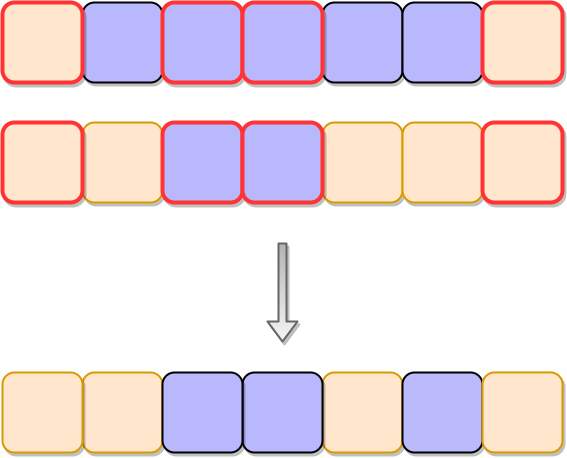
\includegraphics[width=0.5\textwidth]{gfx/UniformCrossover.png}
			        \caption{Uniform crossover example. Note that the highlighted elements are present in both individuals.}

			    \end{figure}

			\end{itemize}

		\subsubsection{In neural networks}

			If binary representations and crossovers are among the most widely studied, it is not quite the case with neural networks in genetic algorithms (probably because the revival of the field happened not many years ago).

			Some parameters (\textit{hyperparameters}, because their values are fixed before the training phase) to tune are the number of hidden layers, or neurons per layer, or the learning rate.

			For the first two, one could do something along the lines of the binary crossovers we just explained: take some layer sizes from one parent and the rest from the other, have the child get as many hidden layers as the average of its parents, etc. Perhaps we want to keep the numbers inside tolerance intervals, so we should check after each operation too.

			To pass learning rates on, maybe a simple average would do. Given that we don't have prior knowledge about the function we are trying to optimize--only that it has a global optimum somewhere--, it would be a reasonable strategy: if the optimum is between two values, an average would keep us in range; if not, we would not have known anyway.

\newpage

	\subsection{Mutation}

		Evolution needs some diversity, and what we have not done with selection and crossover, we must do with mutations in the offspring.
		Again, the mutation operator can take many forms, so we will restrict ourselves to what is applicable.

		\subsubsection{In binary representation}

			The easiest way to mutate a vector of binary elements is to randomly flip one or more of them i.e. write 1 where there was 0 and viceversa. Both the amount of flips and the probability of a mutation rule how much diversity is introduced.

		\subsubsection{In neural networks}

			When dealing with quantities, such as the number of layers or of neurons per layer, the simplest thing to do is to add or subtract. A more frequent mutation could be to just alter the number of neurons in one (or more than one) layer either by a fixed amount or by using a probability distribution (gaussian noise, for instance). A much rarer mutation--for its impact in the structure of the network--could involve a slight change in the number of layers.


	\subsection{Replacement}

		The act of combining the old population and the freshly-created offspring into a new population for the next generations has a great significance in the final outcome of the algorithm. Let us start reviewing the two categories of genetic algorithms according to the magnitude of the replacement:

		\begin{itemize}

			\item
			Steady-state: only a few parents--typically two--are selected for reproduction in each generation, and the offspring they yield replace the same amount of individuals in the original population.

			\item
			Generational: the whole previous population is displaced by a newly created group.

		\end{itemize}

		Because these categories are not strict, we could have a genetic algorithm that ranks halfway between the two: not all the previous individuals have to be replaced. We usually make this decision with the help of additional criteria: imagine that we lump together all the individuals and sort them by fitness; all offspring could be better than the best old individual, and thus the entire population would be replaced, but it might very well not be the case, and end up with a mix of old and new.

		The way in which we choose to do the replacement causes, along with the selection procedure, a certain degree of \textit{selective pressure} \cite{selection-ga}. Selective pressure characterizes the extent to which better individuals are prioritized in the evolution stages of the algorithm

